\documentclass[14pt,xcolor=pdftex,dvipsnames,table]{beamer}\usepackage[]{graphicx}\usepackage[]{color}
%% maxwidth is the original width if it is less than linewidth
%% otherwise use linewidth (to make sure the graphics do not exceed the margin)
\makeatletter
\def\maxwidth{ %
  \ifdim\Gin@nat@width>\linewidth
    \linewidth
  \else
    \Gin@nat@width
  \fi
}
\makeatother

\definecolor{fgcolor}{rgb}{0.345, 0.345, 0.345}
\newcommand{\hlnum}[1]{\textcolor[rgb]{0.686,0.059,0.569}{#1}}%
\newcommand{\hlstr}[1]{\textcolor[rgb]{0.192,0.494,0.8}{#1}}%
\newcommand{\hlcom}[1]{\textcolor[rgb]{0.678,0.584,0.686}{\textit{#1}}}%
\newcommand{\hlopt}[1]{\textcolor[rgb]{0,0,0}{#1}}%
\newcommand{\hlstd}[1]{\textcolor[rgb]{0.345,0.345,0.345}{#1}}%
\newcommand{\hlkwa}[1]{\textcolor[rgb]{0.161,0.373,0.58}{\textbf{#1}}}%
\newcommand{\hlkwb}[1]{\textcolor[rgb]{0.69,0.353,0.396}{#1}}%
\newcommand{\hlkwc}[1]{\textcolor[rgb]{0.333,0.667,0.333}{#1}}%
\newcommand{\hlkwd}[1]{\textcolor[rgb]{0.737,0.353,0.396}{\textbf{#1}}}%

\usepackage{framed}
\makeatletter
\newenvironment{kframe}{%
 \def\at@end@of@kframe{}%
 \ifinner\ifhmode%
  \def\at@end@of@kframe{\end{minipage}}%
  \begin{minipage}{\columnwidth}%
 \fi\fi%
 \def\FrameCommand##1{\hskip\@totalleftmargin \hskip-\fboxsep
 \colorbox{shadecolor}{##1}\hskip-\fboxsep
     % There is no \\@totalrightmargin, so:
     \hskip-\linewidth \hskip-\@totalleftmargin \hskip\columnwidth}%
 \MakeFramed {\advance\hsize-\width
   \@totalleftmargin\z@ \linewidth\hsize
   \@setminipage}}%
 {\par\unskip\endMakeFramed%
 \at@end@of@kframe}
\makeatother

\definecolor{shadecolor}{rgb}{.97, .97, .97}
\definecolor{messagecolor}{rgb}{0, 0, 0}
\definecolor{warningcolor}{rgb}{1, 0, 1}
\definecolor{errorcolor}{rgb}{1, 0, 0}
\newenvironment{knitrout}{}{} % an empty environment to be redefined in TeX

\usepackage{alltt}

% Specify theme
\usetheme{Madrid}
% See deic.uab.es/~iblanes/beamer_gallery/index_by_theme.html for other themes
\usepackage{caption}
\usepackage[comma, sort&compress]{natbib}
\usepackage{graphicx}
\usepackage{amsmath}
\bibliographystyle{agsm}
% Specify base color
\usecolortheme[named=OliveGreen]{structure}
% See http://goo.gl/p0Phn for other colors

% Specify other colors and options as required
\setbeamercolor{alerted text}{fg=Maroon}
\setbeamertemplate{items}[square]

% Title and author information
\title{Using Eviews}
\author{Rob Hayward}
\IfFileExists{upquote.sty}{\usepackage{upquote}}{}


\begin{document}

\begin{frame}
\titlepage
\end{frame}

\begin{frame}{Outline}
\tableofcontents
\end{frame}

\section{Import data}
\begin{frame}{Copy and Paste}
\graphicspath{{./Figures/}}
\frametitle{Import Data}
\begin{center}
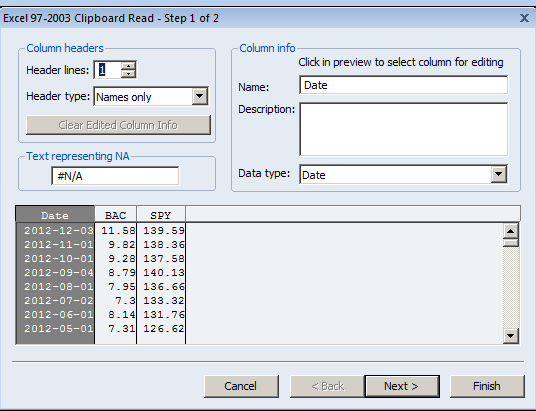
\includegraphics[height = 2.8in]{Import}
\end{center}
\end{frame} 


\begin{frame}{Calculate Returns}
\graphicspath{{./Figures/}}
\frametitle{Return Code}
"Quick", "Generate Series" or, 
\begin{center}
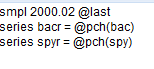
\includegraphics[height = 1.5in]{Returncode}
\end{center}
\end{frame} 

\begin{frame}{Return Series}
\graphicspath{{./Figures/}}
\frametitle{Return Series}
\begin{center}
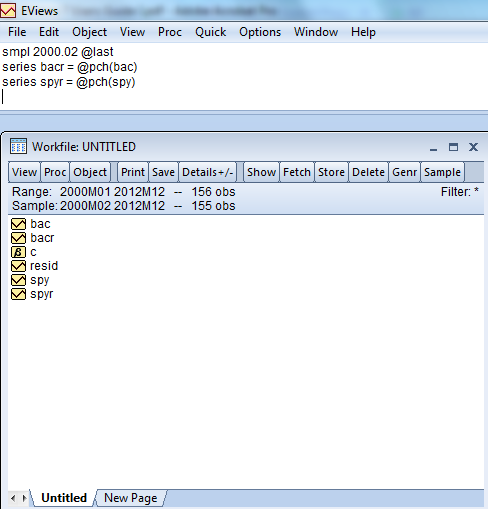
\includegraphics[height = 3.0in]{Returncodefull}
\end{center}
\end{frame} 

\begin{frame}[fragile]{Samples}
You can sample from a smaller range of data.  This can be used to test the stabilty of the parameters or is necessary to compute lags. 
\begin{verbatim}
smpl 2000.01 2012.12
@first @last
@all
\end{verbatim}
\end{frame}

\begin{frame}{Equations}
\graphicspath{{./Figures/}}
\begin{center}
\framebox{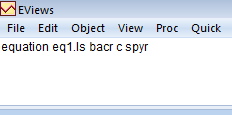
\includegraphics[width = 1.5in]{equation}}
\end{center}

$C$ is the constant\\
$(-1)$ will lag the variable\\
No need to specify the error
\end{frame}

\section{$R^2$}
\begin{frame}{R Squared (p. 13)}
The total variance of the dependent variable is called the total sum of squares (TSS).  This can be split into 
\begin{itemize}[<+-| alert@+>]
\item Explained sum of squares or sum of squares of the regression (ESS)
\item Residual sum of squares (RSS)
\end{itemize}
\pause
\begin{align*}
R^2 &= 1 - \frac{RSS}{TSS} = 1 - \frac{RSS}{RSS + ESS}\\
R^2 &= 1 - \frac{\hat{\varepsilon}'\hat{\varepsilon}}{(y - \bar{y})'(y - \bar{y})}
\end{align*}
\begin{equation}
u = \hat{\varepsilon}
\end{equation}
\end{frame}

\begin{frame}{Adjusted R Squared (p. 13)}
The $R^2$ can be considered a measure of \emph{goodness of fit}.  However, the more variables that you add the smaller the $R^2$. The \emph{Adjusted R Squared} ($\bar{R}^2$) will make a penalty for adding variables. 

\begin{equation}
\bar{R}^2 = 1 - (1 - R^2) \times \frac{(T - 1)}{(T - K)}
\end{equation}
where $T$ is the total number of observations and $K$ is the number of variables. 
\end{frame}


\section{Confidence intervals on coefficients}
\begin{frame}{Coefficient Estimates}
Remember that the estimates of the coefficients will depend on the sample
\begin{itemize}[<+-| alert@+>]
\item A different sample will give a different estimate
\item We want to know how reliable the estimates will be under different samples
\item $\beta$ is a random variable.  If OLS (\emph{Gauss-Markov} assumptions hold)
\begin{itemize}
\item $\hat{\beta_1} \sim N (\beta_1, \sigma_{\beta_1}^2)$
\end{itemize}
\pause
If we assume a normal distribution we can carry out hypothese tests about coefficients like $\beta_1$
\end{itemize}
\end{frame}

\begin{frame}{Variance of Coefficient estimates}
\graphicspath{{./Figures/}}
\begin{center}
\framebox{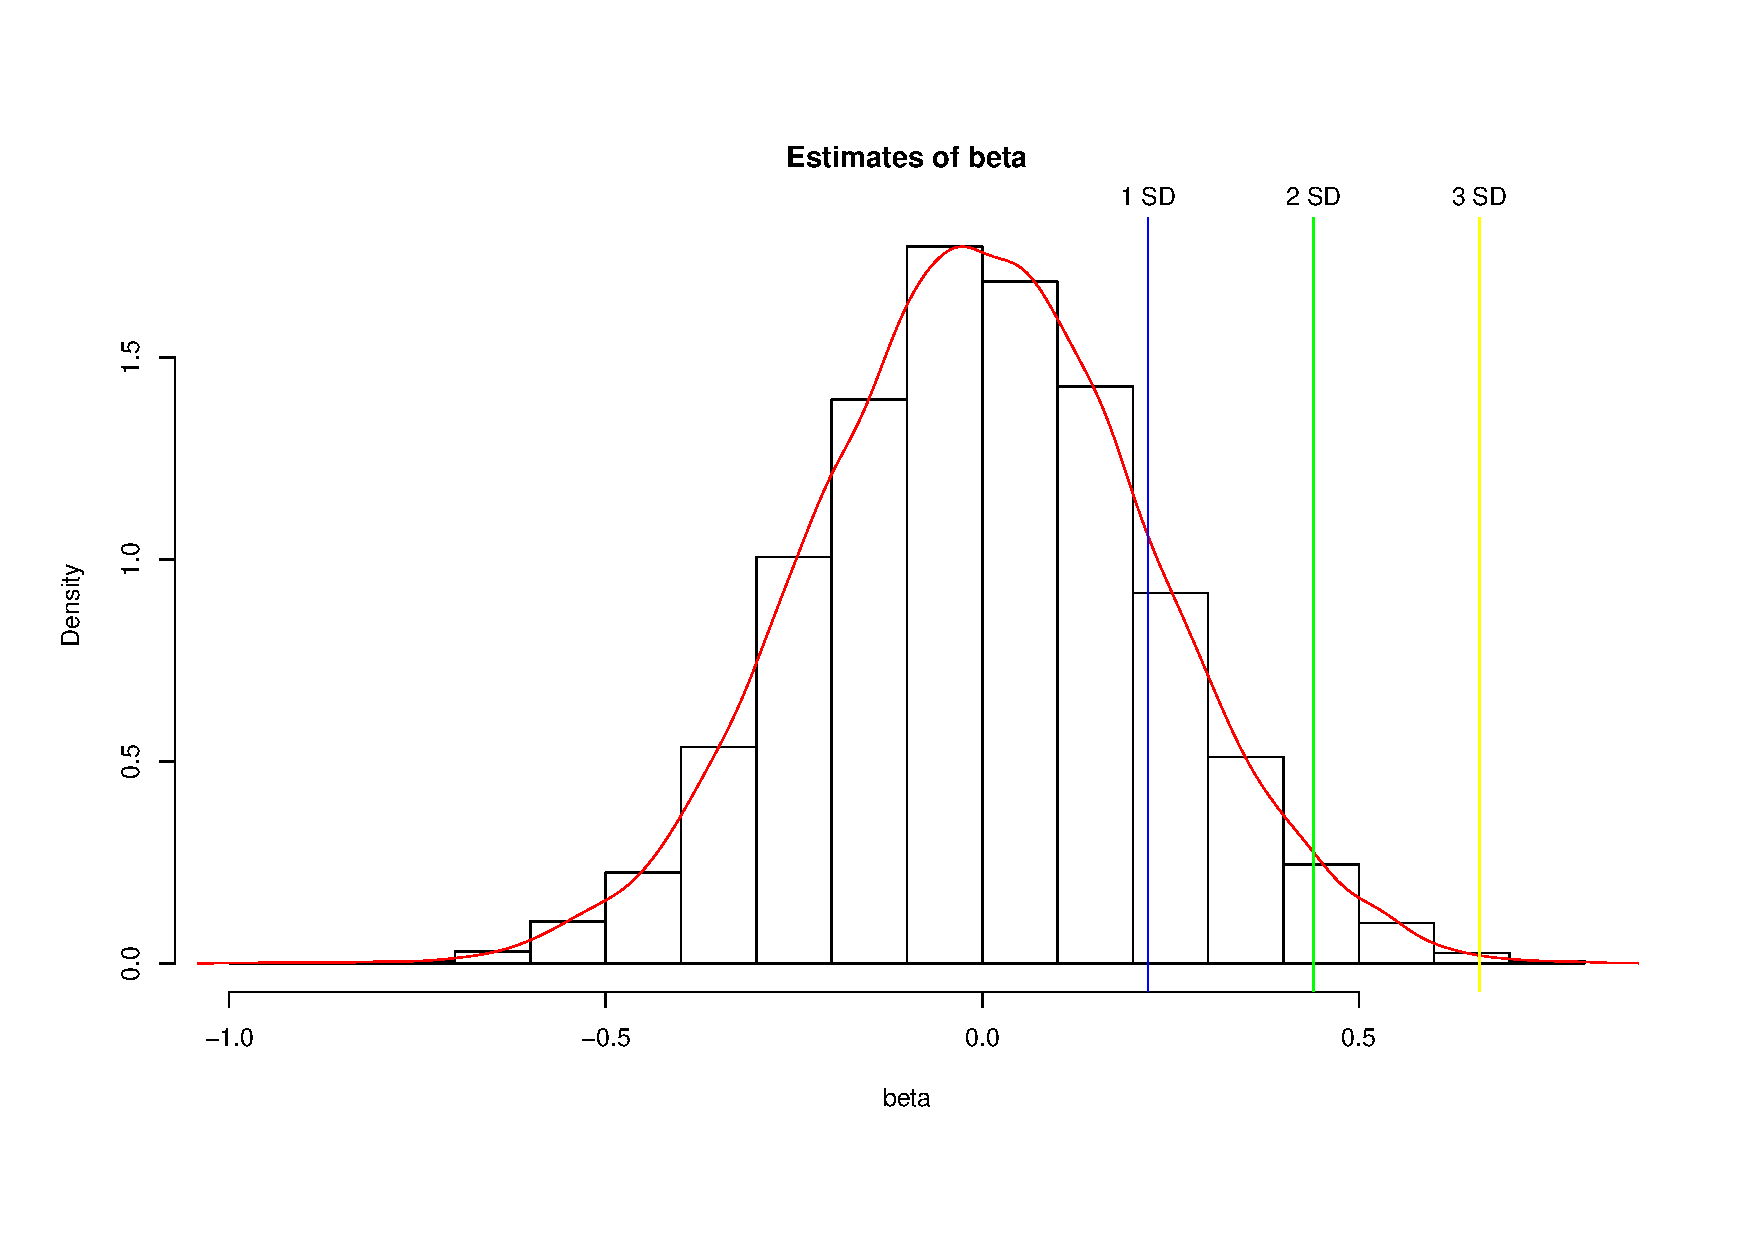
\includegraphics[width = 4.4 in]{Coef}}
\end{center}
\end{frame}

\begin{frame}{Hypothesis tests of Coefficients p.14}
Hypothese tests are conducted using the t-statistic
\begin{block}{}
$\text{t-stat} = \frac{\text{estimator} - \text{hypothesised value}}{\text{standard error of the estimator}}$\\ 
\vskip 0.5cm
$t = \frac{\hat{\beta_1}-\beta_{1,0}}{SE(\hat{\beta_1})}$\\
\vskip 0.5cm 
Need to estimate the standard deviation of the coefficient estimate
\end{block}
\end{frame}

%\begin{frame}{Estimating the distribution of the parameter estimate}
%Covariance matrix of estimated coefficiencts is
%$Var(b) = s^2(X'X)^{-1}$\\
%$s^2 = \frac{\hat{\varepsilon}'\hat{\varepsilon}}{(T - k)}$\\
%$\hat{\varepsilon} = y - Xb$\\
%$SE(\hat{\beta_1}) = \sqrt{Var(b)^2}$
%\end{frame}

\begin{frame}{Eview output 1}
\graphicspath{{./Figures/}}
\frametitle{Standard Errors}
\begin{center}
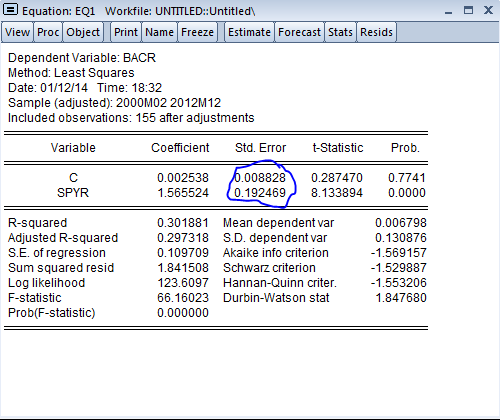
\includegraphics[height = 3 in]{Se}
\end{center}
\end{frame}

\begin{frame}{Eview output 2}
\graphicspath{{./Figures/}}
\frametitle{Standard Errors}
\begin{center}
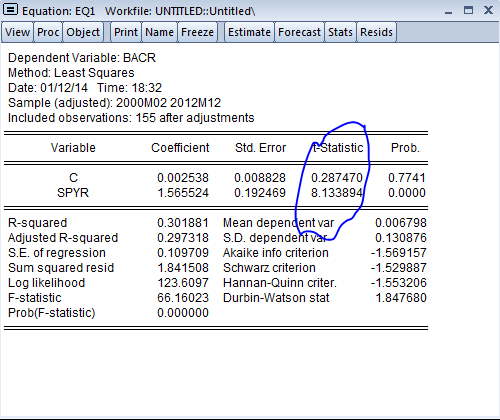
\includegraphics[height = 3 in]{tstat}
\end{center}
\end{frame}

\begin{frame}{Eview output 3}
\graphicspath{{./Figures/}}
\frametitle{Standard Errors}
\begin{center}
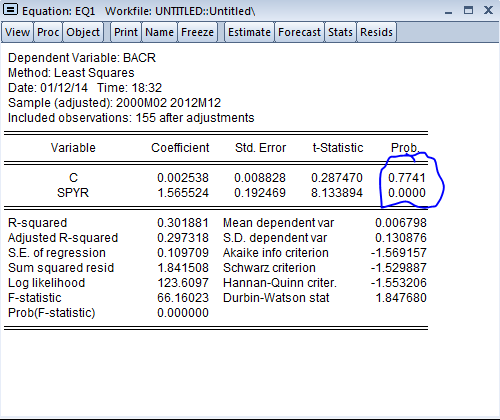
\includegraphics[height = 3 in]{pval}
\end{center}
\end{frame}


\section{Durbin-Watson}
\begin{frame}{Durbin Watson}
This is a test of \emph{first order autocorrelation}\\
If 
$Y_t = a + b X_t + u_t$\\
and \\
$u_t = \rho u_{t-1} + v_t$\\
DW tests 
\begin{align*}
H0:& \rho = 0\\
H1:& \rho > 0
\end{align*}
H0 - There is no first order autocorrelation
\end{frame}

\begin{frame}{Durbin Watson test}
The test is 
\begin{align*}
DW =& 2 - 2 \frac{\sum_{t = 2}^T \hat{u}_t \hat{u}_{t-1}}{\sum_{t=1}^T \hat{u_t}^2}\\
DW =& 2(1 - \hat{\rho})
\end{align*}
DW statistics close to two suggest no autocorrlation of the residuals.
\end{frame}

\begin{frame}{Durbin-Watson Output}
\graphicspath{{./Figures/}}
\begin{center}
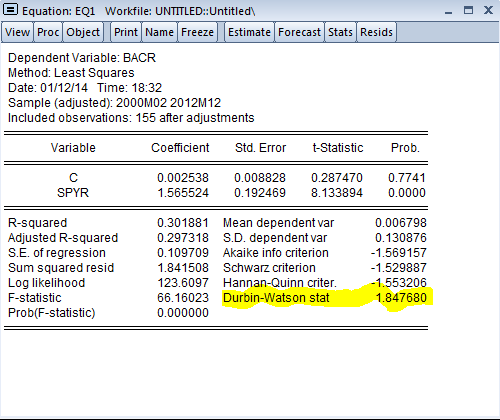
\includegraphics[height = 3 in]{DW}
\end{center}
\end{frame}


\section{Residuals}
\begin{frame}{Residual Tests}
Inspection and tests of the residuals will allow us to assess whether there are problems with the model
\begin{itemize}[<+-| alert@+>]
\item Residuals should be \emph{White Noise}
\item $u =\sim N(0, \sigma^2)$
\item Tests for autocorrelation
\item Tests for hetroskedsasticity
\item Tests for normal distribution
\end{itemize}
\end{frame}

\begin{frame}{Residual Output}
\graphicspath{{./Figures/}}
\frametitle{Standard Errors}
\begin{center}
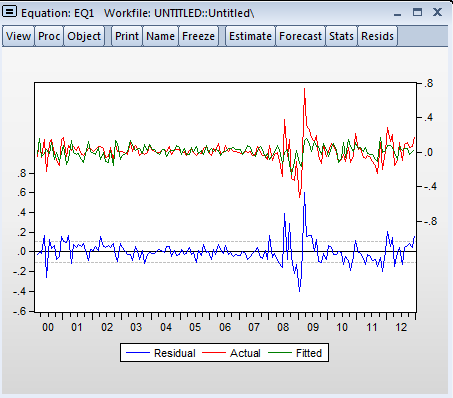
\includegraphics[height = 3 in]{resid}
\end{center}
\end{frame}


\section{Further Reading}
\begin{frame}{Eviews documentation}
\begin{itemize}[<+-| alert@+>]
\item \href{http://www.eviews.com/home.html}{Eviews Website}
\item \href{http://www.eviews.com/Learning/index.html}{Tutorials}
\item User Guide 1 Chapter 11 (p. 315 to 321)
\item User Guide 2 Chapter 18 (p. 1 to 22 )
\end{itemize}
\end{frame}

%\begin{frame}{Bibliography}
%\bibliography{myref}
%\end{frame}
\end{document}
